\subsection{Résultats}

Après les divers corrections au modèles citées dans la partie méthodologie, nous avons lancé une simulation. 
Nous n'avons pas encore eu les données expérimentales et donc nous n'avons pas encore fait l'estimation des paramètres. Nous n'avons pas non plus fait d'étude de sensibilité des paramètres. 
Les résultats exploités et présentés dans ce rapport sont donc des sorties d'une simple simulation en première approche, bien que déjà satisfaisante. Les sorties sont toutes qualitativement très satisfaisantes et pour beaucoup proches des résultats quantitatifs voulus. 

\subsubsection{Cadre de la simulation}

La simulation se fait sur 275 jours, avec un pas de discrétisation d'un jour. Les paramètres utilisés nous ont été donnés par notre client, Pierre Carmier, ils correspondent à des paramètres réalistes et cohérents avec la littérature scientifique pour ce type de modèle et de plante. Les données environnementales correspondent à des données réelles qui nous ont aussi été fournies par le client.


\subsubsection{Résultats considérés}

Nous considérerons les sorties suivantes :

\begin{itemize}

	\item \textbf{La masse du grain (fig.~\ref{fig:resultatGrain}):} C'est la donnée la plus importante et la plus intéressante à mesurer qui correspond à la récolte de céréale. On attend une valeur autour de 1000.
	
	\item \textbf{Le LAI (fig.~\ref{fig:resultatLAI}):} C'est l'indice de surface foliaire, décrit précédemment, il est directement lié à la masse du feuillage vert. On le préfère à ce dernier car les valeurs qu'il atteint classiquement sont connues : on attend une valeur entre 5 et 6.
	
	\item \textbf{La masse des tiges (fig.~\ref{fig:resultatStem}):} Son profil est intéressant à suivre car il est lié à deux moments critiques : le temps de montaison (temps à partir duquel la biomasse est allouée aux tiges en priorité) et un second temps de remobilisation de la biomasse de la tige (en même temps que celle des feuilles vertes) qui se transforme en grain.
	
	\item \textbf{La quantité d'eau dans le sol (fig.~\ref{fig:resultatWater}):} Une part importante du modèle est la simulation du comportement de l'eau dans le sol. Il est donc intéressant de voir de façon globale comment la quantité d'eau sur la couche du sol considérée évolue.
	
	\item \textbf{L'indice de stress hydrique (fig.~\ref{fig:resultatStressH}):} Il permet de voir à quel moment la plante manque d'eau et les influences que cela a sur la croissance de la plante.
	
	\item \textbf{L'indice de stress thermique (fig.~\ref{fig:resultatStressT}):} De même il permet de voir l'influence de la température sur la croissance de la plante.

\end{itemize}

\begin{figure}[H]

\begin{center}
 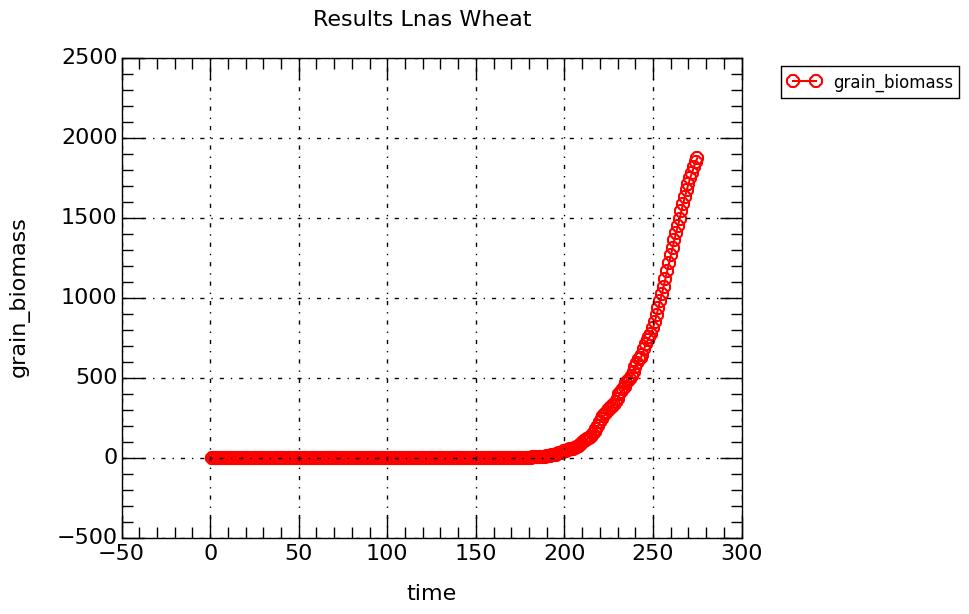
\includegraphics[scale = 0.67]{./img/grain.png}
 \caption{Biomasse de grain en fonction du temps.}
 \label{fig:resultatGrain}
\end{center}

\end{figure}

\begin{figure}[H]

\begin{center}
 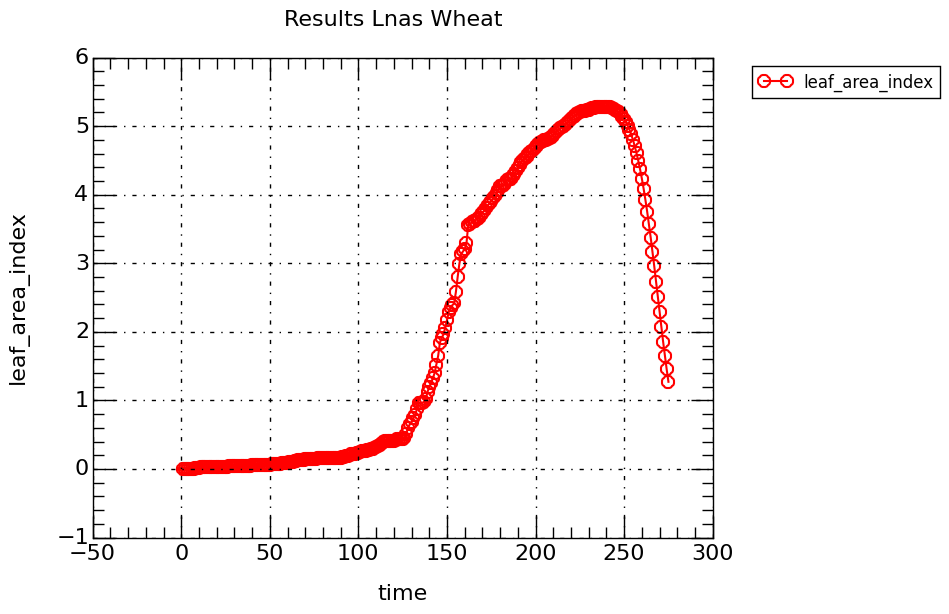
\includegraphics[scale = 0.67]{./img/LAI.png}
 \caption{Indice LAI en fonction du temps.}
 \label{fig:resultatLAI}
\end{center}

\end{figure}

\begin{figure}[H]

\begin{center}
 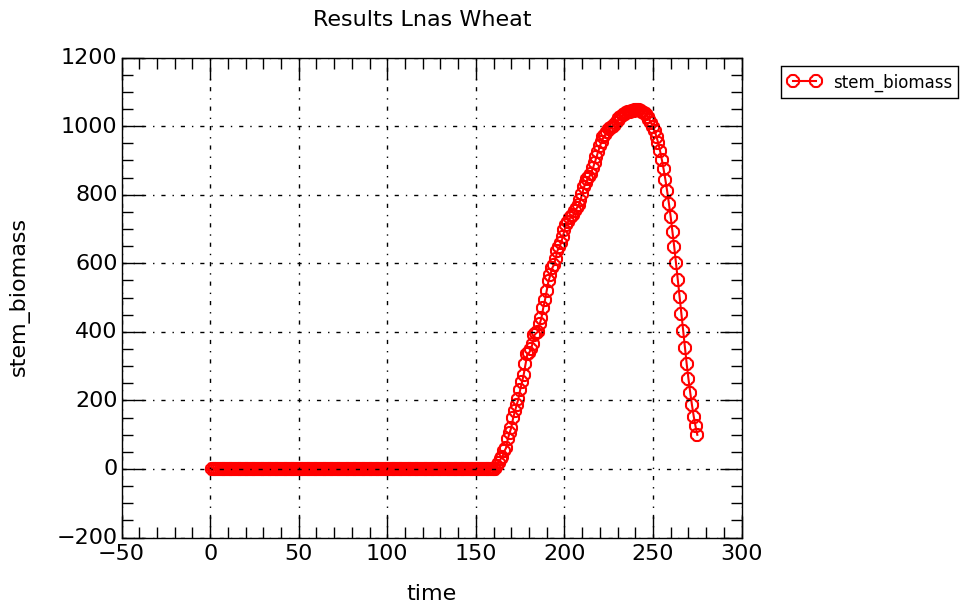
\includegraphics[scale = 0.67]{./img/stem.png}
 \caption{Biomasse de la tige en fonction du temps.}
 \label{fig:resultatStem}
\end{center}

\end{figure}

\begin{figure}[H]

\begin{center}
 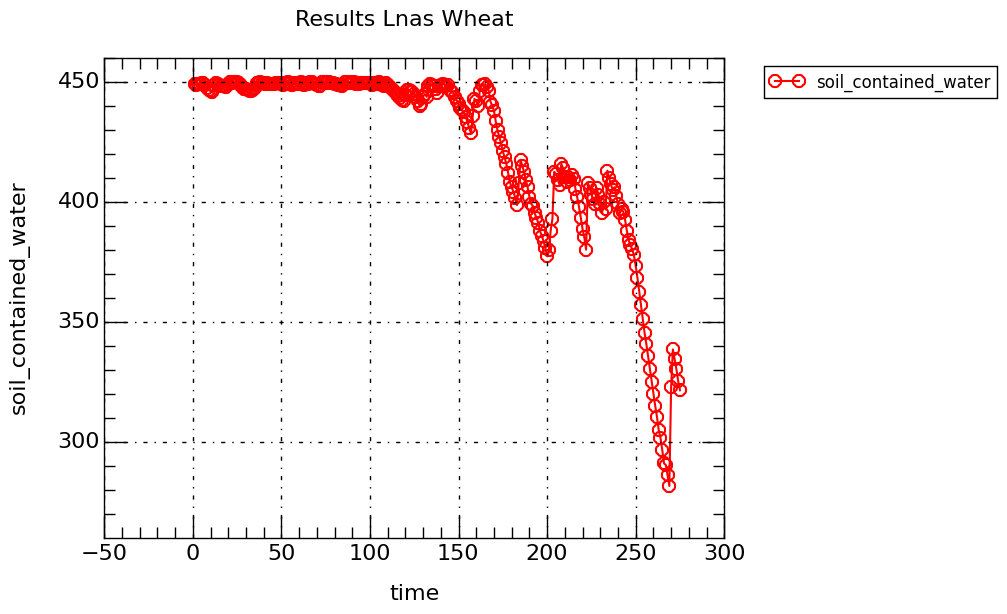
\includegraphics[scale = 0.67]{./img/water.png}
 \caption{Quantité d'eau dans la couche de sol considérée.}
 \label{fig:resultatWater}
\end{center}
\end{figure}

\begin{figure}[H]

\begin{center}
 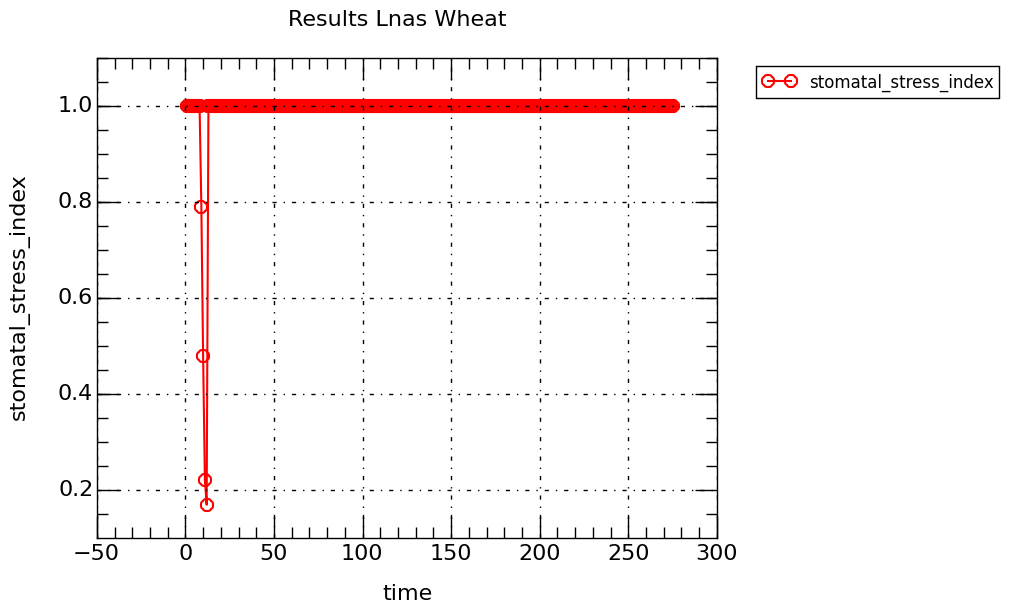
\includegraphics[scale = 0.67]{./img/waterStress.png}
 \caption{Indice de stress hydrique en fonction du temps.}
 \label{fig:resultatStressH}
\end{center}

\end{figure}

\begin{figure}[H]

\begin{center}
 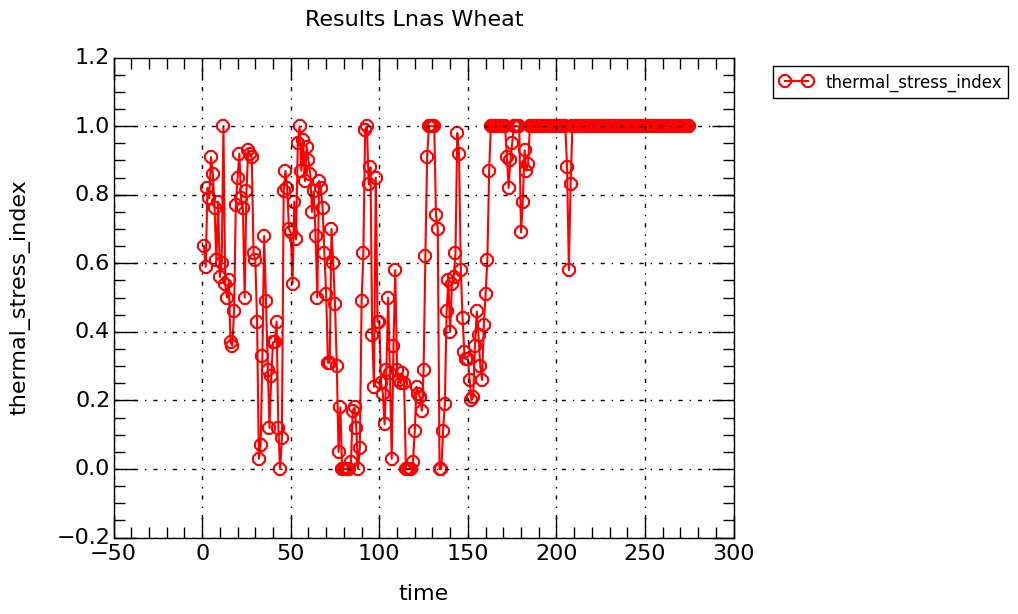
\includegraphics[scale = 0.67]{./img/thermicStress.png}
 \caption{Indice de stress thermique en fonction du temps.}
 \label{fig:resultatStressT}
\end{center}

\end{figure}

\subsubsection{Résultats et commentaires}

Pour ces différentes sorties, nous avons eu les résultats suivants :

\begin{itemize}
	\item \textbf{La masse du grain :} Nous avons un comportement qualitatif totalement cohérent : une croissance rapide et tardive de la quantité de grain. Cependant cette croissance dure trop longtemps et la quantité de biomasse du grain au moment de la récolte atteint des valeurs autour de 2000 au lieu de 1000. Les causes plausibles sont expliquées dans la partie méthodologie.
	
	\item \textbf{Le LAI :} Le résultat est à la fois très cohérent qualitativement et quantitativement. Le profil de la courbe correspond à celui qu'on trouve expérimentalement : croissance très rapide, croissance rapide, pic puis décroissance rapide. Et les valeurs maximum obtenues sont bien entre 5 et 6.
	
	\item \textbf{La masse des tiges :} Le comportement est cohérent et correspond à celui attendu : une croissance rapide à partir du temps de montaison puis une décroissance rapide avec la remobilisation et la sénescence. Il nous faudrait comparer avec des données expérimentales pour le quantitatif.
	
	\item \textbf{La quantité d'eau dans le sol :} Les réserves d'eau dans le sol sont larges au début et ne sont mises à mal par la plante que vers la fin alors qu'elle est déjà à maturité. Les paramètres environnementaux ne rendent pas la question de l'eau cruciale dans cette simulation : elle est abondante.
	
	\item \textbf{L'indice de stress hydrique :} La conclusion précédente est confirmée. La plante ne ressent à aucun moment de stress hydrique, à part un court épisode au départ dû à la longueur insuffisante de la racine mais rapidement corrigée. Pour mieux apprécier et évaluer la partie simulation de l'eau, on pourrait essayer le modèle avec des données environnementales qui présenteraient des périodes de sécheresse qui rendraient la question de l'eau plus cruciale.
	
	\item \textbf{L'indice de stress thermique :} Plus prévisible et direct que le stress hydrique, il est directement lié à la température. La simulation commence en hiver, le stress peut être ressenti avec des températures inférieures à 10, les épisodes de stress thermique sont donc surtout marqués en début de simulation, où ils peuvent ralentir la croissance de la plante, mais leur occurrence est normale en hiver et pas suffisamment sévère dans nos données pour empêcher la croissance normale de la plante.
\end{itemize}

Ainsi nous avons obtenu des résultats très satisfaisants qualitativement qui montrent que le modèle est fonctionnel et cohérent. Les comportements de sortie sont ceux attendus. La quantité de grain obtenue en sortie reste trop importante pour être réaliste et nous devons améliorer le modèle sur ce point. Les autres résultats quantitatifs sont satisfaisants.
